\chapter{Pipelines \& Algorithms}
\pagenumbering{arabic} \setcounter{page}{13}

This section examines the two most widely used pipelines that are used to generate OTUs and ASVs. The first pipeline employs the Divisive Amplicon Denoising Algorithm (DADA), which produces the ASVs. The second utilises the Unweighted UniFrac Algorithm (implemented through Mothur), which is used to make OTUs.

\section{DADA}
The DADA is a hierarchical clustering algorithm that works by removing PCR-amplified artefacts from the sequenced reads. The algorithm's goal is to infer the genotypes of the microbes present in the sample along with their error rates. The algorithm operates until the genotypes and errors rates from the noisy sequenced data converge to a mutually consistent set. DADA was compared against the AmpliconNoise algorithm, which it outperformed on various parameters. However, DADA assumes each error to be statistically independent, and there might be a case where a single DNA might produce many artefacts which could induce non-independent errors.\newline

\subsection{Divisive Amplicon Denoising Algorithm}
The p-values ($p_{y}$,$p_{\alpha}$) forms the basis of the algorithms, through which it iteratively updates the partition set of sequence B and the nucleotide error probabilities T. After t iterations the partition set of sequence and the nucleotide error probabilities updates to $B^{t}$ and $T^{t}$. There are three levels of nesting in the algorithm and each of them is repeated until convergence. Beginning with $T^{0}$, the maximum likelihood nucleotide error probabilities are provided partition $B^{0}$ in a unique cluster, and the outermost loop recursively upgrade B \& T until T converges. The following loop begins with the partition, $B^{t}$ = $B^{0}$, and attaches blocks to $B^{t}$ until the $p_{y}$ and $p_{\alpha}$ does not permit rejection of model at common significance levels. If statistically significant families exist that supports both p-values, then a new cluster is formed. After this inner-most loop boosts the probability by reassigning each sequence to the block that would generate the most considerable required amount of reads of that sequence, this proceeds until sequences discontinue renewing clusters.\newline

\begin{figure}
  \centering
  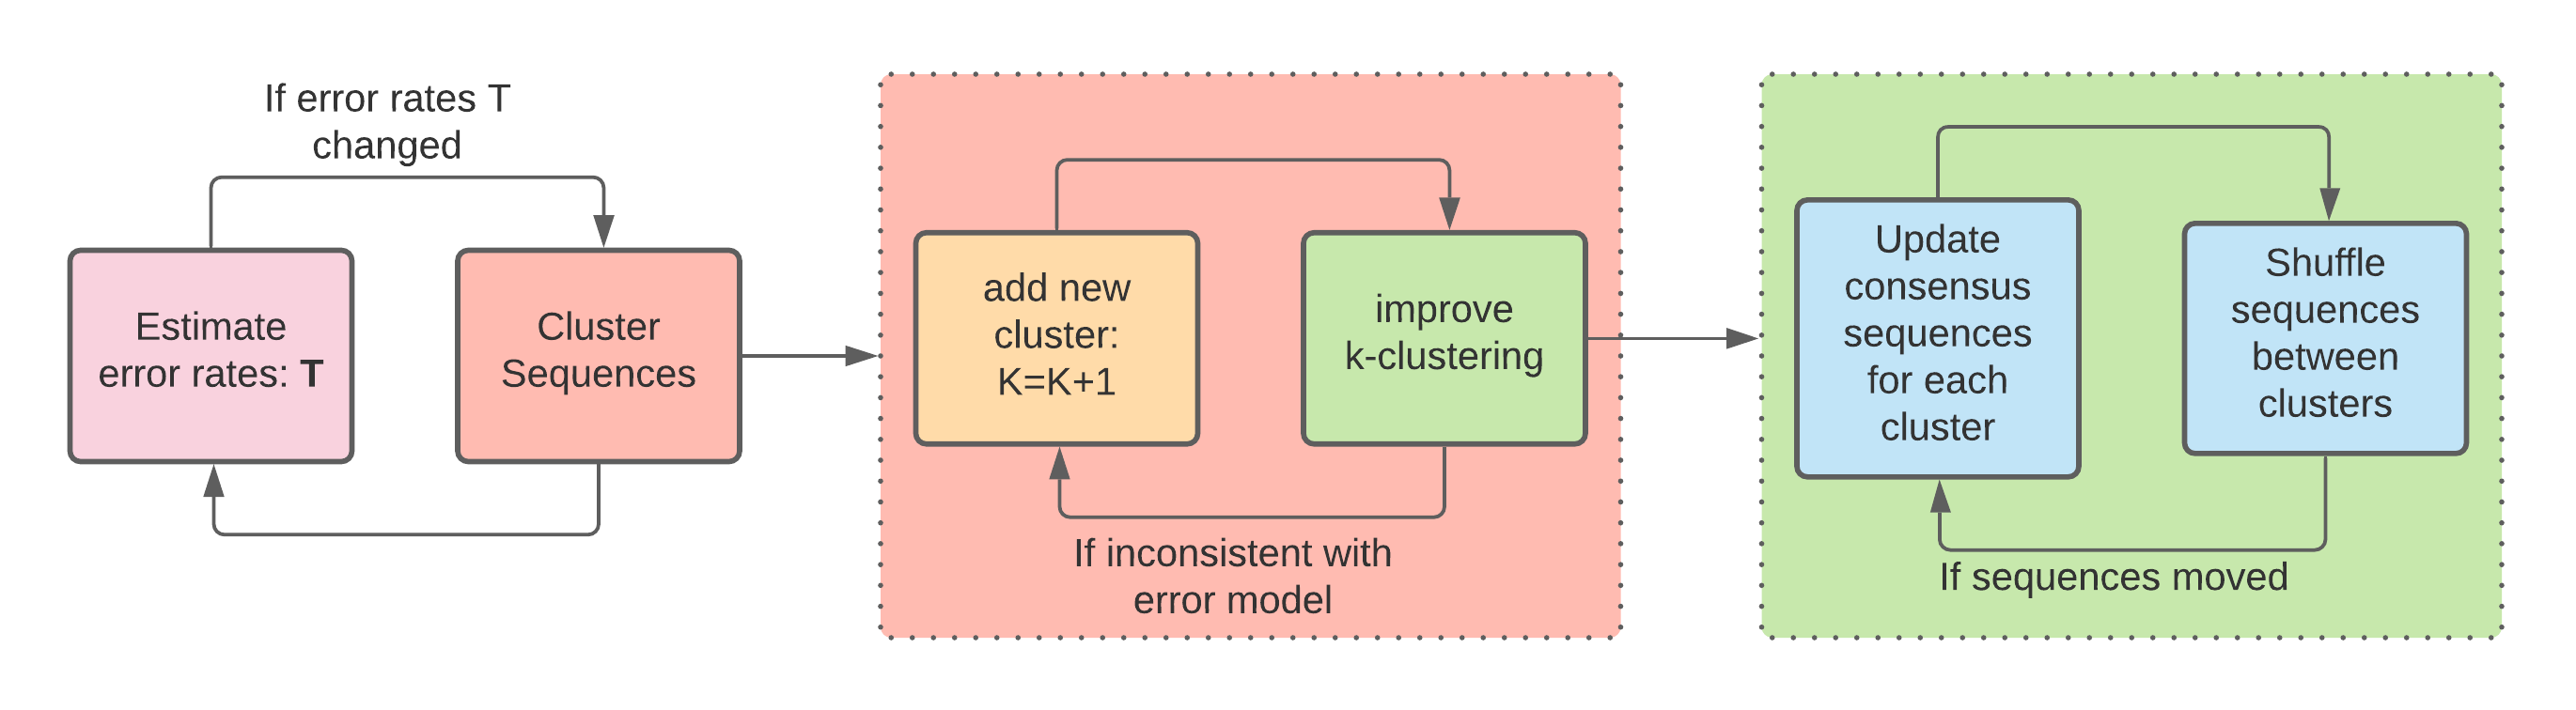
\includegraphics[width=15cm]{../Figure4.png}
  \caption{Schematic representation of DADA algorithm}
  \label{fig:figure4}
\end{figure}

The DADA is currently running in its second version, available as an R library, "DADA2". The DADA2 employ a novel QC-informed model of Illumina amplicon errors. The DADA2 pipeline commences with the command "fastqFilter()", which trims adaptors, removes short sequences and ambiguous bases. DADA can apply this to both paired-end and single-end reads. This step is accompanied by the "derep()" function, which performs the dereplication of the data. Lastly, the DADA's de-ionising algorithm is implemented, which is explained in  \ref{fig:figure4}; it estimates genotypes and calculates errors. One can also remove chimaeras by performing Needleman-Wunsch global alignment using the function "isBimeraDenovo()". The complete pipeline of DADA2 is given in Appendix-1.

\section{MOTHUR}
The MOTHUR is a comprehensive tool written in C++ using Object-Oriented-Programming (OOPs) fundamentals. It integrates the algorithms from previous packages/tools, including SONS, DOTUR, and TreeClimber. MOTHUR operates on various clustering algorithms such as the nearest neighbour, OptiCLust, Unweighted-pair group method using average linkages (UPGMA). Here I discuss the OptiCLust algorithm, which is the default algorithm of MOTHUR that produces OTUs.

\subsection{OptiClust}

\begin{figure}[!hb]
  \centering
  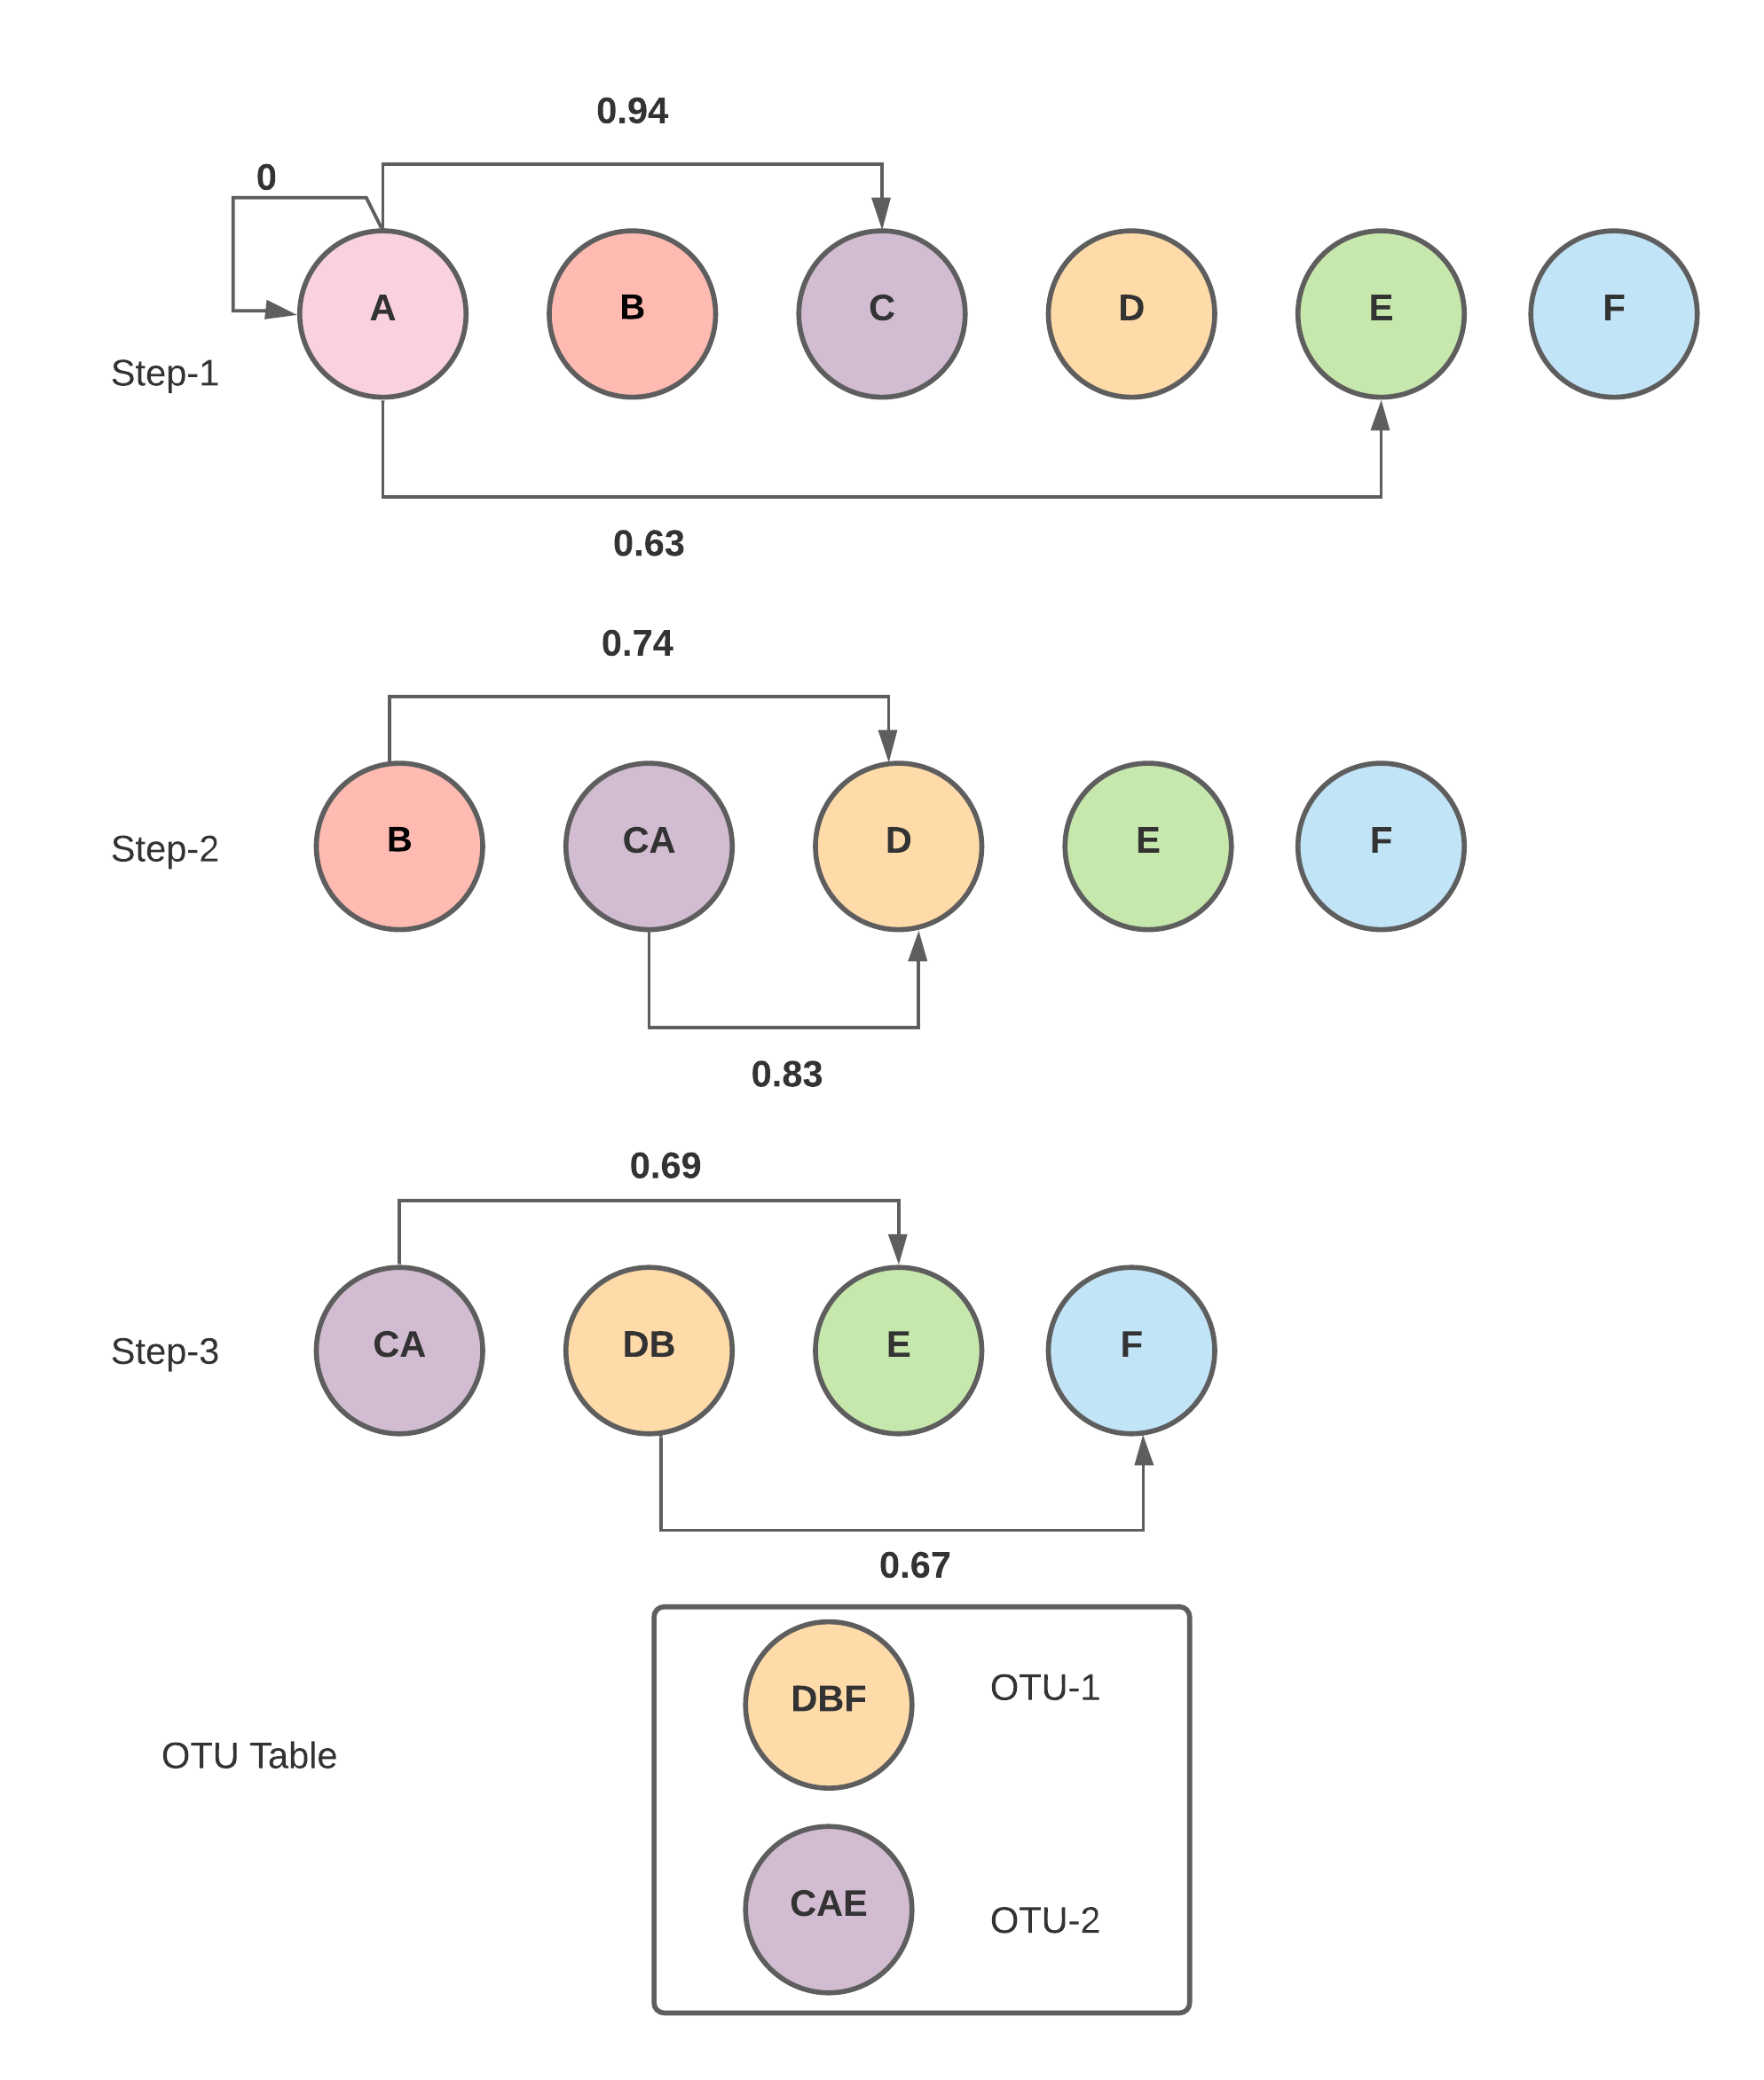
\includegraphics[width=10cm, height=12cm]{../Figure5.png}
  \caption{Schematic representation of OptiClust algorithm}
  \label{fig:figure5}
\end{figure}

The OptiCLust begins by calculating the pairwise distance between all the sequences. It then removes the sequences having a pairwise distance less than a threshold. Once the filtered set is obtained, it seeds by assigning each sequence a distinct OTU. The convergence initiates by calculating Matthew's Correlation Coefficient (MCC) between the first singleton OTU and the other sequences. The MCC for singleton OTU itself is zero; therefore, it chooses the different available sequences that increase the MCC value. If the change in the MCC is the same between the two sequences then, it randomly selected either of the two. This step is repeated until the entire sequence set is converted into OTUs [Figure \ref{fig:figure5}]. To initiate OptiClust algorithm requires either a phylip-formatted distance matrix or a column-formatted distance matrix. The "cluster" command initiates the clustering process that creates the OTUs.